\documentclass[document.tex]{subfiles} 
\begin{document}

\clearpage
\subsection{Отображение в виде графа}
Адаптер формирующий граф из примитивов символьной алгебры логики именуется
GraphAdapter. Его описывание представлено в листинге~\ref{lst:graph}.

\begin{listing}[ht]
\begin{minted}[linenos=true]{python}
class GraphAdapter(AbstractAdapter):
    public_properties = ('graph', 'max_distance')
    default_content_type = 'image/png'

    def default_method(self):
        graph = self.graph
        labels_dict = dict()
        for graph_node in graph.nodes_iter():
            graph_type = graph.node[graph_node]['type']
            if graph_type == 'input':
                labels_dict[graph_node] = graph_node
            elif graph_type == 'output':
                labels_dict[graph_node] = 'output'
        pyplot.figure(figsize=(6, 4), dpi=100)
        graph_pos = random_layout(graph)
        draw_networkx_nodes(graph, pos=graph_pos, node_size=640)
        draw_networkx_edges(graph, pos=graph_pos, width=0.5, alpha=0.3)
        draw_networkx_labels(graph, pos=graph_pos, font_size=8, 
                             labels=labels_dict)

        pyplot.xlim(-0.05, 1.05)
        pyplot.ylim(-0.05, 1.05)
        pyplot.axis('off')
        _, tmpfile = mkstemp(suffix='.png')
        pyplot.savefig(tmpfile)
        return tmpfile

\end{minted}
\caption{Программное описание класса адаптера графов}
\label{lst:graph}
\end{listing}

Пример применения адаптера построения графов к устройству (в данном случае,
эквиваленция) иллюстрируется кодом, представленным в
листинге~\ref{lst:graphgen}.

\begin{listing}[ht]
\begin{minted}{pycon}
>>> from circuitry.adapters.graph import GraphAdapter                   
>>> from circuitry.devices.cmp import DeviceEq 
>>>
>>> device_eq = DeviceEq(strobe_signals='v:1', first_signals='f:2',
...                      second_signals='s:2', output_signals='o:2',
...                      strobe_signals_subs=dict(v0=1))
>>>
>>> GraphAdapter(device_eq).default_method()
'/tmp/tmpNs3x52.png'
\end{minted}
\caption{Генерация графа}
\label{lst:graphgen}
\end{listing}

\clearpage
Файл, полученный применением адаптера
представлен на рисунке~\ref{fig:adapters_graph}.

\begin{figure}[here]
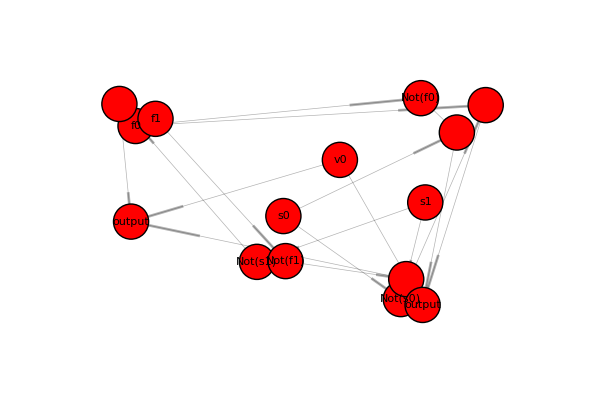
\includegraphics[width=1\linewidth]{adapters_graph}
\caption{Представление устройства эквиваленции в виде графа}
\label{fig:adapters_graph}
\end{figure}

\end{document}